\documentclass{article}\usepackage[]{graphicx}\usepackage[]{color}
%% maxwidth is the original width if it is less than linewidth
%% otherwise use linewidth (to make sure the graphics do not exceed the margin)
\makeatletter
\def\maxwidth{ %
  \ifdim\Gin@nat@width>\linewidth
    \linewidth
  \else
    \Gin@nat@width
  \fi
}
\makeatother

\definecolor{fgcolor}{rgb}{0.345, 0.345, 0.345}
\newcommand{\hlnum}[1]{\textcolor[rgb]{0.686,0.059,0.569}{#1}}%
\newcommand{\hlstr}[1]{\textcolor[rgb]{0.192,0.494,0.8}{#1}}%
\newcommand{\hlcom}[1]{\textcolor[rgb]{0.678,0.584,0.686}{\textit{#1}}}%
\newcommand{\hlopt}[1]{\textcolor[rgb]{0,0,0}{#1}}%
\newcommand{\hlstd}[1]{\textcolor[rgb]{0.345,0.345,0.345}{#1}}%
\newcommand{\hlkwa}[1]{\textcolor[rgb]{0.161,0.373,0.58}{\textbf{#1}}}%
\newcommand{\hlkwb}[1]{\textcolor[rgb]{0.69,0.353,0.396}{#1}}%
\newcommand{\hlkwc}[1]{\textcolor[rgb]{0.333,0.667,0.333}{#1}}%
\newcommand{\hlkwd}[1]{\textcolor[rgb]{0.737,0.353,0.396}{\textbf{#1}}}%

\usepackage{framed}
\makeatletter
\newenvironment{kframe}{%
 \def\at@end@of@kframe{}%
 \ifinner\ifhmode%
  \def\at@end@of@kframe{\end{minipage}}%
  \begin{minipage}{\columnwidth}%
 \fi\fi%
 \def\FrameCommand##1{\hskip\@totalleftmargin \hskip-\fboxsep
 \colorbox{shadecolor}{##1}\hskip-\fboxsep
     % There is no \\@totalrightmargin, so:
     \hskip-\linewidth \hskip-\@totalleftmargin \hskip\columnwidth}%
 \MakeFramed {\advance\hsize-\width
   \@totalleftmargin\z@ \linewidth\hsize
   \@setminipage}}%
 {\par\unskip\endMakeFramed%
 \at@end@of@kframe}
\makeatother

\definecolor{shadecolor}{rgb}{.97, .97, .97}
\definecolor{messagecolor}{rgb}{0, 0, 0}
\definecolor{warningcolor}{rgb}{1, 0, 1}
\definecolor{errorcolor}{rgb}{1, 0, 0}
\newenvironment{knitrout}{}{} % an empty environment to be redefined in TeX

\usepackage{alltt}
\usepackage{natbib}
\usepackage{color}
\usepackage[dvipsnames,svgnames*]{xcolor}
\usepackage{array}
\usepackage[hidelinks]{hyperref}
\usepackage[font=small,skip=5pt]{caption}
\usepackage[aboveskip=2pt]{subcaption}
\usepackage{graphicx}
\usepackage{amsmath}
\usepackage{dsfont}
\usepackage[]{algorithm2e}
\usepackage{amsthm}
\usepackage{amsfonts}
\usepackage{url}
\usepackage{ulem}
\usepackage{afterpage}
\usepackage{bbm}
\numberwithin{equation}{section}
\IfFileExists{upquote.sty}{\usepackage{upquote}}{}
\begin{document}

\tableofcontents

\section{Bayesian Inference}

\subsection{Bayes' Rule}

In Bayesian statistics, we are interested in making inferences about an unknown parameter $\theta$ using what is known as the posterior distribution, $p(\theta | y)$, where $y$ is our observed data. Bayes' rule provides a form for this distribution, 

\begin{equation}
\label{BR1}
p(\theta | y) = \frac{p(y | \theta) p(\theta)}{p(y)},
\end{equation}

which shows that the posterior can be found by taking the product of the likelihood, $p(y | \theta)$ and the prior distribution, $p(\theta)$, and normalising with a constant $p(y)$. In practice $p(y)$ is unknown and can be found from 

\begin{equation}
\label{BR2}
p(y) = \int_\theta p(y | \theta) p(\theta) d \theta.
\end{equation}

Finding the value of $p(y)$ is often the most difficult part of working with Bayesian statistics. In some simple models, this integration can be solved analytically, but for most models of interest it is intractable and we can only work with the un-normalised version

\begin{equation}
\label{BR3}
p(\theta | y)^* = p(y | \theta) p(\theta).
\end{equation}

This work will concern itself with two of the methods used in the case where (\ref{BR2}) is intractable, exact methods such as MCMC, which will be discussed later in this section as well as an approximation method known as Variational Bayes which appears in section two.

\subsection{Exact Bayesian Computation}

\textbf{1. Numerical Integration}\newline

It might be tempting to numerically approximate (\ref{BR2}) by evaluting the integrand over a grid and applying methods such as the Trapezoid Rule or Adaptive Quadrature. These may be suitable for integration in a low dimension, but if we have a grid with $G$ points in one dimension, then a two dimensional integration requires $G^2$ points, and a three dimensional integration requires $G^3$ points. In general, the computational time increases exponentially with the dimension of $\theta$ in numerical integration. In almost all cases of interest, $\theta$ is a high-dimensional vector which makes numerical integration prohibitively expensive. This is known as the curse of dimensionality, where the difficulty of the problem increases quickly with the dimension of $\theta$ and requires us to use more sophisticated methods.\newline

\textbf{2. Importance Sampling} \newline

Candidate Density
Accept Reject
Good candidate is hard but useful
VB as a candidate \newline

\textbf{3. Gibbs Sampling}\newline

Breaks down into simple problems
Becomes linear instead of exponential
Exact sampling \newline

\textbf{4. Metropolis Hastings within Gibbs}\newline

Gibbs only works exactly on some problems
Approximation within Gibbs
Also can benefit from VB

\section{Variational Bayes}

\subsection{Estimation as an optimisation problem}

In the event that our dataset is too large, or our model is too complex, for MCMC to converge within a reasonable time frame we must resort to approximation. One important question that might be asked then is \textit{`How do I measure how good my approximation is?'}. If two distributions come from the same family, one might consider the difference in the parameters, but it is trivial to come up with distributions with slight parameter differences and vastly different regions of probability mass. Consider the difference between a $\mathcal{N}(0, 0.1)$ and a $\mathcal{N}(0.5, 0.1)$ distribution, the change in mean is only $0.5$ but there is little overlap in the densities. Further, large values for the variance allow large changes in mean with very little change in the resulting densities. If the distributions come from different families it is almost impossible to use parameters to measure the degree of closeness between two distributions. Instead we must move from the parameter space to the distribution space, where one measure of the difference between distributions $p(\theta)$ and $q(\theta)$ is the Kullback-Leibler (KL) divergence \citep{Kullback1951}, defined by

\begin{equation}
\label{KL-def}
KL[q(\theta)||p(\theta)] = \int q(\theta) \ln \left( \frac{q(\theta)}{p(\theta)}\right) d\theta.
\end{equation}

KL divergence is a non-negative, assymetric measure of the difference between $p(\theta)$ and $q(\theta)$ that will equal zero if and only if $p(\theta) = q(\theta)$ almost everywhere. It has origins in information theory, and can be interpreted as: \textit{`Given that I know $p(\theta)$ for some $\theta \in \Theta$, how much extra information is required, on average, to know the value of $q(\theta)$?'} There are examples of the literature of approximations with other measures of divergence, such as \citet{Minka2001} introducting Expectation Propogation, which minimises the reverse measure $KL[p(\theta)||q(\theta)]$, which was extended to Power-EP in \citet{Minka2004}, which aims to minimisea the more general $\alpha-\mbox{divergence}$ \citep{Amari1985}.
\vspace{3mm}

\begin{figure}[hb]
\begin{knitrout}
\definecolor{shadecolor}{rgb}{0.969, 0.969, 0.969}\color{fgcolor}
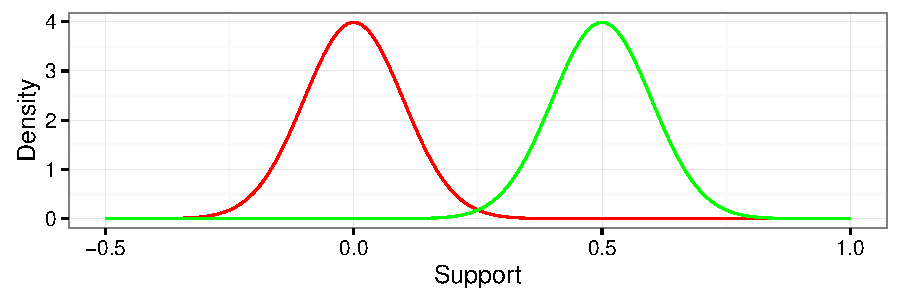
\includegraphics[width=\maxwidth]{figure/klnorm-1} 

\end{knitrout}
\caption{Red: A Normal(0, 0.1) distribution. Green: A Normal(0.5, 0.1) distribution.}
\end{figure}

\newpage

Variational Bayes aims to find the approximating distribution, $q(\theta | \lambda)$, that minimises $KL[q(\theta | \lambda)||p(\theta |y)]$. This approximating distribution is parameterised by a $\lambda$ vector, each element of which may be a function of $y$, the hyperparameters of the prior distribution, and even of other elements in $\lambda$. The optimal approximation, in the sense of having the minimum KL divergence with the posterior, can be derived by beginning with the unknown constant, $\ln(p(y))$.
\begin{align}
\ln(p(y)) &= \int_{\theta} q(\theta|\lambda) \ln(p(y)) d\theta \nonumber \\
&= \int_{\theta} q(\theta|\lambda) \ln  \left( \frac{p(y, \theta)}{p(\theta | y)} \right) d\theta \nonumber \\
&= \int_{\theta} q(\theta|\lambda) \ln  \left( \frac{p(y, \theta)}{p(\theta | y)} \frac{q(\theta|\lambda)}{q(\theta|\lambda)}\right) d\theta \nonumber \\
&= \int_{\theta} q(\theta|\lambda) \ln  \left( \frac{q(\theta|\lambda)}{p(\theta | y)}\right) + \ln \left( \frac{p(y, \theta)}{q(\theta|\lambda)} \right) d\theta \nonumber \\
&= \int_{\theta} q(\theta|\lambda) \ln  \left( \frac{q(\theta|\lambda)}{p(\theta | y)}\right) d\theta + \int_{\theta} q(\theta|\lambda) \ln \left( \frac{p(y, \theta)}{q(\theta|\lambda)} \right) d\theta \nonumber \\
&= KL [q(\theta||\lambda) || p(\theta | y)] + \mathcal{L}(q(\theta | \lambda), y) \nonumber
\end{align}


where 

\begin{align}
\mathcal{L}(q(\theta|\lambda), y) &= \int_{\theta} q(\theta|\lambda) \ln \left( \frac{p(y, \theta|\lambda)}{q(\theta|\lambda)} \right) d\theta \nonumber \\
&=  \int_{\theta} q(\theta|\lambda) \ln (p(y, \theta|\lambda)) d\theta -  \int_{\theta} q(\theta|\lambda) \ln (q(\theta|\lambda)) d\theta. \label{ELBO}
\end{align}

Hence we have that
\begin{equation}
\label{VBKL}
KL [q(\theta|\lambda) || p(\theta | y)] = \ln(p(y)) - \mathcal{L}(q(\theta | \lambda), y).
\end{equation}

From (\ref{VBKL}) it is clear that by maximising $\mathcal{L}(q(\theta | \lambda), y)$ with respect to $q(\theta|\lambda)$ the KL divergence between the unknown true posterior $p(\theta|y)$ and the approximating distribution $q(\theta|\lambda)$ will be minimised.
Hence the Variational Bayes solution will be to maximise the Evidence Lower Bound (ELBO), $\mathcal{L}(q(\theta|\lambda), y)$, in (\ref{ELBO}).

\subsection{Mean Field Variational Bayes}

Mean Field Variational Bayes (MFVB) has origins in the physics literature \citep{Chandler1987} and uses the assumption that the approximation dististribution factorises, 
\begin{equation}
\label{mf1}
q(\theta|\lambda) = \prod_i q_i(\theta_i | \lambda_i).
\end{equation}

This assumption is known as the Mean Field assumption and is has been widely used as it greatly simplifies maximisation of the ELBO (\citealp{Jordan1999}; \citealp{Bishop2006}). Each component $\theta_i$ may be a scalar or a vector, and $\lambda_i$ is the component of the $\lambda$ vector that parameterises the relevant factor $q_i(\theta_i |\lambda_i)$. From here, we will use the shorthand notation that $q_i = q_i(\theta_i|\lambda_i)$ and $q_{\setminus i} = \prod_{j\neq i}q_j$. Maximising the ELBO with respect to $q_i$ is analytically involved but computationally simple, as (\ref{ELBO}) can be expressed as a function of $q_i$ only and then maximised with respect to each $q_i$ individually.

\begin{align}
\mathcal{L}(q_i) &= \int_{\theta} q_i q_{\setminus i} \ln (p(y, \theta)) d\theta - \int_{\theta} q_{i}q_{\setminus i} \ln (q_{i}q_{\setminus i}) d\theta \nonumber \\
&= \int_{\theta_i}\int_{\theta_{\setminus i}} q_{i}q_{\setminus i} ( \ln (p(y, \theta)) - \ln(q_{i})) d\theta_i d\theta_{\setminus i} - \int_{\theta_i}\int_{\theta_{\setminus i}} q_{i}q_{\setminus i} \ln (q_{\setminus i}) d\theta_i d\theta_{\setminus i}  \nonumber \\
&= \int_{\theta_{i}} q_{i} \left( \int_{\theta_{\setminus i}} q_{\setminus i} \ln (p(y, \theta )) d\theta_{\setminus i} - \ln(q_i) \right) d\theta_i \nonumber \\
&- \int_{\theta_{\setminus i}} q_{\setminus i} \ln(q_{\setminus i}) d\theta_{\setminus i} \label{mf2}\\
&= \int_{\theta_{1}} q_{i} \ln \left( \frac{\exp(  \mathbb{E}_{q_{\setminus i}} [\ln(p(y,\theta))])}{q_i} \right) d\theta_i + c \nonumber \\
&= -KL (q_i || \exp( \mathbb{E}_{q_{\setminus i}} [\ln(p(y,\theta))])) + c \label{mf2.2}
\end{align}

as the rightmost component of (\ref{mf2}) is constant with respect to $q_i$.

We can see that by holding $q_{\setminus_i}$ fixed, we can maximise the ELBO with respect to $q_i$ by minimising the KL Divergence between $q_i$ and $\exp( \mathbb{E}_{q_{\setminus i}} [\ln(p(y,\theta))])$ in (\ref{mf2.2}). This is easily done by setting

\begin{equation}
\label{mf3}
q(\theta_i | \lambda_i) \propto\exp( \mathbb{E}_{q_{\setminus i}} [\ln(p(y,\theta))]).
\end{equation}

If the likelihood and prior for $\theta_i$ form an exponential family conjugate pair, then this maximisation proceeds by keeping the distributional family constant and simply updating the parameters $\lambda_i$. Otherwise, we can find the optimal distributional family for any $q_i$ by taking the log-joint density and then ignoring any term that doesn't depend on $\theta_i$. Next, take the expectation of any remaining $\theta_{j \neq i}$ and then match to the kernel of a known distribution. If it does not match a known distribution, we may need to make a further approximation $\tilde{q_i(\theta_i|\lambda_i)}$ which has a recognizable distribution. One method as used in \citet{Friston2006} uses a Laplace approximation for the otherwise unrecognizable $q_i(\theta_i | \lambda_i)$ with reasonable results.

These steps are almost the same as those used to find a conditional distribution $p(\theta_i | \theta_{j \neq i}, y)$, with dependence on other parameters replaced by their expectations. Hence, the optimal approximating family for $\theta_i$, $q(\theta_i | \lambda_i)$, will come from the same distributional family as the conditional distribution $p(\theta_i | \theta_{j \neq i}, y)$, if it exists in a recognisable form such as the exponential family. Deriving the updating algorithm for MFVB takes more analytical effort than finding the conditionals for a Gibbs MCMC scheme, as we must then find the values of each $\lambda_i$ implied by (\ref{mf3}), which are often a function of $\lambda_{j \neq i}$ through the expectations.
\vspace{5mm}

Given these optimal distributional families, an algorithm that cycles through all of the $\lambda_i$ and sets each to its maximising value is known as a coordiante ascent algorithm. The algorithm must continuously iterate between each parameter until $\mathcal{L}(q(\theta | \lambda), y)$ converges with some pre-defined threshold noting that the $\lambda$ may depend on each other. If $\lambda$ has dimension $k$, the algorithm follows below.

\vspace{2mm}

\begin{algorithm}[H]
 \SetKwInOut{Input}{Input}
 \Input{Log Joint Density}
 \KwResult{Mean Field Approximation}
 Initialise $\lambda$ randomly\;
 \While{Not converged}{
  \For{$i =  1$ \KwTo $k$}{
      Hold $\lambda_{j \neq i}$ fixed\;
      Use (\ref{mf3}) to match $q(\theta_i|\lambda_i)$ to a known distribution\;
      Update $\lambda_i$ using the most recent values of $\lambda_{j \neq i}$\;
     }
 }
 \caption{Coordinate Ascent for MFVB}
  \label{alg:algorithm1}
\end{algorithm}

\subsection{Stochastic Gradient Ascent}

In many cases, the posterior is too complex to be captured by a factorising approximation and we desire our distribution $q(\theta | \lambda)$ to capture dependence between parameters. In this case, the easy maximisation in MFVB is unavailable, and we must resort to what is called Stochastic Variational Bayes (SVB) using a gradient ascent algorithm developed by \citet{Paisley2012} and \citet{Hoffman2013}.

To maximise the function $\mathcal{L}(q(\theta | \lambda), y)$ we can take the derivative of $\mathcal{L}(q(\theta | \lambda), y)$ with respect to $\lambda$ and use the updating step:

\begin{equation}
\label{SGA1}
\lambda^{(m)} = \lambda^{(m-1)} + \rho^{(m)} \nabla_{\lambda} \mathcal{L}(q(\theta | \lambda^{(m-1)}), y),
\end{equation}

where $\nabla_{\lambda}\mathcal{L}(q(\theta | \lambda^{(m-1)}), y)$ is the vector of partial derivatives of $\mathcal{L}(q(\theta | \lambda^{(m-1)}), y)$ with respect to each element of $\lambda$. This update requires initial values $\lambda^{(0)}$ and some sequence $\rho^{(m)}$. If $\rho^{(m)}$ is chosen to satisfy the following conditions, it is a Robbins-Monro sequence and the algorithm is guaranteed to converge to a local maximum.

\begin{align}
\lim_{m \xrightarrow[]{} \infty} \rho^{(m)} &= 0 \nonumber \\
\sum_{m=1}^{\infty} \rho^{(m)} &=  \infty \nonumber \\
\sum_{m=1}^{\infty} (\rho^{(m)})^2 &<  \infty. \nonumber
\end{align}

Whilst a global maximum is desired, the ELBO can have a problem specific shape that makes finding the global maximum extremely difficult, as we do not know how many stationary points exist. The dimension of the ELBO is the dimension of the $\lambda$ vector, which is often much greater than the dimension of the parameters $\theta$ so a grid search is suspect to the curse of dimensionality. To alleiviate this problem, we can start the algorithm at a range of initial values choose the converged value with the highest value of the ELBO. 

SVB does not provide the family of the the optimal approximating distribution, unlike under the mean field assumption. To run SVB we may need to try many approximating distributions and then choose the $q(\theta | \lambda)$ that has the highest ELBO, and hence lowest KL divergence to the true posterior. We must restrict the approximation to distributions that satisfy the condition that the order of differentation of the ELBO with respect to $\lambda$ and integration with respect to $\theta$ are interchangable. In this case, we can calculate derivatives of the ELBO.

\begin{align}
\nabla_{\lambda} \mathcal{L}(q(\theta | \lambda), y) &=  \nabla_{\lambda} \int_{\theta} q(\theta | \lambda) \left( \ln (p(y, \theta)) - \ln(q(\theta | \lambda)) \right) d\theta \nonumber \\
&=   \int_{\theta} \nabla_{\lambda}[  q(\theta | \lambda) \left( \ln (p(y, \theta)) - \ln(q(\theta | \lambda)) \right)] d\theta \label{SGA2} \\
&=  \int_{\theta}  q(\theta | \lambda) \nabla_{\lambda}[( \ln (p(y, \theta)) - \ln(q(\theta | \lambda))] d\theta \nonumber \\ 
&+ \int_{\theta} \nabla_{\lambda} [q(\theta | \lambda)] \left( \ln (p(y, \theta)) - \ln(q(\theta | \lambda)) \right) d\theta \label{SGA3}
\end{align}

Note that the first integral on the right hand side of (\ref{SGA3}) equals 0 as

\begin{equation}
\int_{\theta}  q(\theta | \lambda) \nabla_{\lambda}[( \ln (p(y, \theta))] d\theta = 0
\end{equation}

and

\begin{align}
\int_{\theta} - q(\theta | \lambda) \nabla_{\lambda}[ \ln(q(\theta | \lambda))] d\theta &= - \int_{\theta} \frac{\nabla_{\lambda}q(\theta | \lambda)}{q(\theta | \lambda)} q(\theta | \lambda) d\theta \nonumber \\
&=  -  \nabla_{\lambda}\int_{\theta} q(\theta | \lambda) d\theta \nonumber \\
&=  0 \nonumber
\end{align}

Then we continue from (\ref{SGA3}) with 

\begin{align}
\nabla_{\lambda} \mathcal{L}(q(\theta | \lambda), y) &=  \int_{\theta} \nabla_{\lambda} [q(\theta | \lambda)] \left( \ln (p(y, \theta)) - \ln(q(\theta | \lambda)) \right) d\theta \nonumber \\
&=   \int_{\theta} q(\theta | \lambda)  \nabla_{\lambda} [\ln(q(\theta | \lambda))]\left( \ln (p(y, \theta)) - \ln(q(\theta | \lambda)) \right)d\theta \nonumber \\
&= E_q \left(  \nabla_{\lambda} [\ln(q(\theta | \lambda))]\left( \ln (p(y, \theta)) - \ln(q(\theta | \lambda)) \right) \right). \label{SGA4}
\end{align}

We can compute a Monte-Carlo estimate of (\ref{SGA4}) by 

\begin{equation}
\label{SGA5}
\nabla_{\lambda}\mathcal{L}(q(\theta | \lambda)) \approx \frac{1}{S}\sum_{s=1}^{S} \nabla_{\lambda} [\ln(q(\theta_s | \lambda))] (\ln (p(y, \theta_s)) - \ln(q(\theta_s | \lambda)))
\end{equation}

where $\theta_s$, $s = 1, \dots S$, are simulated from the most recent iteration of  $q(\theta | \lambda)$.

As the distribution $q(\theta | \lambda)$ is specified by the user, the main restriction on the use of SVB is that the log-joint density $\ln(p(y, \theta))$ is able to be evaluated. Running an SVB algorithm involves very little analytical effort unlike MFVB, most of the difficulty is calculating the score function of the approximating distribution,
$\nabla_{\lambda} [\ln(q(\theta_s | \lambda))]$. But as this is part of the approximation and not the true model the code to run this could potentially be re-used in many different models. 

\begin{algorithm}[H]
 \SetKwInOut{Input}{Input}
 \Input{Log Joint Density, Approximation family q}
 \KwResult{Variational Approximation}
 Initialise $\lambda$\;
 \While{Not converged}{
  Simulate $\theta^s$ for $s = 1, \dots S$ from $q(\theta|\lambda^{(m-1)})$\;
  \For{$i =  1$ \KwTo $k$}{
      Calculate $\nabla_{\lambda_i} =  1/S\sum_{s=1}^{S} \nabla_{\lambda_i}[\log(q(\theta^s|\lambda^{(m-1)})](\log(p(\theta^s, y)) - \log(q(\theta^s |\lambda^{(m-1)})))$\;
     }
  Set $\lambda^{(m)} = \lambda^{(m-1)} + \rho^{(m)}  \nabla_{\lambda}$\;
  Set $m = m + 1$\;
 }
 \caption{Gradient Ascent for SVB}
  \label{alg:algorithm2}
\end{algorithm}

\subsection{SVB Extensions}

\textbf{1. AdaGrad} \newline


If the gradient is small, we want the learning rate, $\rho_t$, to be large, and if the gradient is large, we want the learning rate to be small. AdaGrad \citep{Duchi2011} is a method of setting the learning rate to dynamically adapt as the values of the calculated gradients changes. Further, AdaGrad allows the step size of each element of $\lambda$ to move independently of the other elements of $\lambda$. 

If $\nabla_{\lambda}^{(m)}$ is the vector of gradients at iteration $m$, define

\begin{equation}
G^{(m)} = \sum_{i = 1}^{m} \nabla_{\lambda}^{i} (\nabla_{\lambda}^{i})^T,
\end{equation}

the sum of the outer products of the gradients up to iteration $m$. Then set 

\begin{equation}
\label{adagrad}
\rho^{(m)} = \eta \mbox{diag}(G^{(m)})^{-1/2}
\end{equation}

with some preset tuning parameter $\eta$. If we have $k$ elements in $\lambda$, $G^{(m)}$ is a $k \times k$ matrix so we have one element in $\rho^{(m)}$ for each element of $\lambda$. As we only need the diagonal of $G^{(m)}$, this may be calculated in linear time. \newline

\textbf{2. Reparameterisation} \newline

The reparameterisation trick was popularised following \citet{Kingma2013} and allows the gradient of the ELBO to be simplified.

Consider a parameter free auxillary distribution $q(\epsilon)$ and differentiable transformation $f(\cdot,\cdot)$ such that $\theta = f(\epsilon, \lambda)$. Examples include a location-scale transformation from a standard normal or an inverse-CDF transform from a uniform$(0, 1)$ variable. Note that 

$$q_\theta(\theta | \lambda) = q_\epsilon(\epsilon) \left| \frac{d\epsilon}{d\theta} \right| $$

where the parameters that govern the transform $f$ are the same $\lambda$ parameters as in $q(\theta | \lambda)$. Now (\ref{SGA2}) becomes

\begin{align}
\nabla_{\lambda} \mathcal{L}(q(\theta | \lambda), y) &=  \int_{\epsilon} \nabla_{\lambda}[  q(\epsilon) \left( \ln (p(y, f(\epsilon, \lambda))) - \ln(q(f(\epsilon, \lambda) | \lambda) \right)] d\epsilon \nonumber \\
&=  \int_{\epsilon}  q(\epsilon) \nabla_{\lambda} \left[ \ln (p(y, f(\epsilon, \lambda))) - \ln(q(f(\epsilon, \lambda)| \lambda) \right] d\epsilon \label{RP1} \\
&= \int_{\epsilon}  q(\epsilon) \nabla_{\lambda} \left[ \ln (p(y, f(\epsilon, \lambda)) \right] d\epsilon\nonumber
\end{align}

as the second part on the right hand side of (\ref{RP1}) is a score function with expectation equal to zero. This can be estimated using 

\begin{equation}
\label{RP2}
 \mathcal{L}(q(\theta | \lambda), y) \approx  \frac{1}{S}\sum_{s=1}^{S} \nabla_{\lambda} \left[ \ln (p(y, f(\epsilon_s, \lambda))) \right].
\end{equation}

with $\epsilon_s \sim q(\epsilon)$.

\citet{Kingma2015} explore how this reparameterised version can have orders of magnitude lower variance than the estimator in (\ref{SGA5}).


\begin{algorithm}[H]
 \SetKwInOut{Input}{Input}
 \Input{Log Joint Density, Approximation family q}
 \KwResult{Variational Approximation}
 Initialise $\lambda$\;
 \While{Not converged}{
  Simulate $\epsilon^s$ for $s = 1, \dots S$\;
  \For{$i =  1$ \KwTo $k$}{
      Calculate $\nabla_{\lambda_i} =  1/S\sum_{s=1}^{S} \nabla_{\lambda_i}[\log(p(f(\epsilon^s, \lambda^{(m-1)}), y))]$
     }
  Set $\lambda^{(m)} = \lambda^{(m-1)} + \rho^{(m)} \nabla_{\lambda}^{t}$\;
  Set $m = m + 1$\;
 }
 \caption{Gradient Ascent for re-parameterised SVB}
  \label{alg:algorithm3}
\end{algorithm}


$\mbox{ }$\newline \textbf{3. Control Variates} \newline

If reparameterisation is too difficult or otherwise unavailable, \citet{Paisly2012} introduce the use use of control variates to estimate the gradient with reduced variance.

Define

\begin{equation}
\label{CV1}
g(\theta, \lambda, y) =  \nabla_{\lambda} [\ln(q(\theta_s | \lambda))] (\ln (p(y, \theta_s)) - \ln(q(\theta_s | \lambda))),
\end{equation}

the function estimated in (\ref{SGA5}), then for some other function $h$, define

\begin{equation}
\label{CV2}
\hat{g}(\theta, \lambda, y) = g(\theta, \lambda, y) - a(h - \mathbb{E}(h)).
\end{equation}

Then we have that

\begin{equation}
\mathbb{E}(\hat{g}) = \mathbb{E}(g)
\end{equation}

and

\begin{equation}
\label{CV3}
\mbox{Var}(\hat{g}) = \mbox{Var}(g) + a^2 \mbox{Var}(h) - 2a\mbox{Cov}(g, h). 
\end{equation}

Solving the polynomial (\ref{CV3}) in $a$ shows that the variance of $\hat{g}$ is minimised by 

\begin{equation}
\label{CV4}
\hat{a} = \mbox{Cov}(g, h)/\mbox{Var}(h).
\end{equation}

Substituting (\ref{CV4}) into (\ref{CV3}) yields

\begin{equation}
\label{CV5}
\mbox{Var}(\hat{g}) = \mbox{Var}(g) - \mbox{Cov}(g, h)^2/\mbox{Var}(h).
\end{equation}

We need to choose some function $h$ that has a large covariance with $g$. \citet{Ranganath2014} suggests that the an easy option is

\begin{equation}
\label{CV6}
h(\theta, \lambda) = \nabla_{\lambda} [\ln(q(\theta_s | \lambda))].
\end{equation}

As $h$ is a score function, it has an expectation of zero and our estimator becomes

\begin{equation}
\label{CV7}
\nabla_{\lambda} \mathcal{L}(q(\theta | \lambda), y) \approx \frac{1}{S}\sum_{s=1}^{S} \nabla_{\lambda} [\ln(q(\theta_s | \lambda))] (\ln (p(y, \theta_s)) - \ln(q(\theta_s | \lambda)) - \hat{a}),
\end{equation}

where $\hat{a}$ is estimated from the sample variance and covariance of a subset of the $S$ Monte-Carlo draws.

\begin{algorithm}[H]
 \SetKwInOut{Input}{Input}
 \Input{Log Joint Density, Approximation family q}
 \KwResult{Variational Approximation}
 Initialise $\lambda$\;
 \While{Not converged}{
  Simulate $\theta_s$ for $s = 1, \dots S$ from $q(\theta|\lambda^{(m-1)})$\;
  \For{$i =  1$ \KwTo $k$}{
      Calculate $g_{\lambda_i} = 1/S\sum_{s=1}^{S} \nabla_{\lambda_i}[\log(q(\theta^s|\lambda^{(m-1)})](\log(p(\theta^s, y)) - \log(q(\theta^s |\lambda^{(m-1)})))$\;
      Calculate $h_{\lambda_i} = 1/S\sum_{s=1}^{S}\nabla_{\lambda_i}[\log(q(\theta^s |\lambda^{(m-1)}))]$\;
      Use a subset of $S$ to estimate $\hat{a} = \mbox{Cov}(h, g)/\mbox{Var}(g)$\;
      Calculate $\nabla_{\lambda_i} = g_{\lambda_i} - \hat{a} h_{\lambda_i}$\;
     }
  Set $\lambda^{(m)} = \lambda^{(m-1)} + \rho^{(m)}  \nabla_{\lambda}$\;
  Set $m = m + 1$\;
 }
 \caption{Gradient Ascent for SVB with control variates}
  \label{alg:algorithm4}
\end{algorithm}
  
\subsection{AR2 model example}

Consider $T$ observations from an AR(2) model conditioned on $y_1$ and $y_2$,

\begin{equation}
\label{AR2}
y_t = \phi_1 y_{t-1} + \phi_2 y_{t-2} + \epsilon_t \mbox{ for } t = 3,\dots,T,
\end{equation}

where $\epsilon$ are iid $\mathcal{N}(0, \sigma^2)$.

Using the independent priors: 

\begin{align}
p(\phi_1) &\sim \mathcal{N}(\bar{\phi_1}, \tau_{1}) \nonumber \\
p(\phi_2) &\sim \mathcal{N}(\bar{\phi_2}, \tau_{2}) \nonumber \\
p(\sigma^2) &\sim \mathcal{IG} (\mbox{shape} = a, \mbox{ scale} = b), \nonumber
\end{align}

we have a model with zero stationary restrictions which can easily be sampled through a Gibbs MCMC scheme. This exact posterior can be used in comparision with the results of our variational approximations.

The Gibbs conditional distributions are derived in the appendix and are

\begin{align}
p(\phi_1 | \phi_2, \sigma^2, y_{1:T}) &\propto \mathcal{N}(\mu_1^G, \gamma_1^G) \nonumber \\
p(\phi_2 | \phi_1, \sigma^2, y_{1:T}) &\propto \mathcal{N}(\mu_2^G, \gamma_2^G) \nonumber \\
p(\sigma^2 | \phi_1, \phi_2, y_{1:T}) &\propto \mathcal{IG}(shape = \alpha^G,  scale = \beta^G), \nonumber
\end{align}

where

\begin{align}
\mu_1^G &= \frac{\tau_1 (\sum_{t=3}^{T} y_t y_{t-1} - \phi_2 \sum_{t=3}^{T} y_{t-1} y_{t-2}) + \sigma^2 \bar{\phi_1}}
          {\tau_1 \sum_{t=3}^{T} y_{t-1}^2 + \sigma^2} \nonumber \\
\gamma_1^G &= \frac{\sigma^2 \tau_1}{\tau_1 \sum_{t=3}^{T} y_{t-1}^2 + \sigma^2} \nonumber \\
\mu_2^G &= \frac{\tau_2 (\sum_{t=3}^{T} y_t y_{t-2} - \phi_1 \sum_{t=3}^{T} y_{t-1} y_{t-2}) + \sigma^2 \bar{\phi_2}}
          {\tau_2 \sum_{t=3}^{T} y_{t-2}^2 + \sigma^2} \nonumber \\
\gamma_2^G &= \frac{\sigma^2 \tau_2}{\tau_2 \sum_{t=3}^{T} y_{t-2}^2 + \sigma^2} \nonumber \\
\alpha^G &= a + T/2 - 1 \nonumber \\
\beta^G &= b + 1/2 \sum_{t=3}^{T} \left((y_t - \phi_1 y_{t-1} - \phi_2 y_{t-2})^2 \right).  \nonumber
\end{align}

100 data points are simulated from the model in (\ref{AR2}) with true values of $\phi_1 = 0.8, \phi_2 = 0.15$ and $\sigma^2 = 2$. These values were chosen to induce a strong dependence between the $\phi$ parameters as it is close to the non-stationary region of $\phi_1 + \phi_2 > 1$. The resulting posterior is sampled with 100,000 draws from Gibbs MCMC, discarding the first 20\% of all draws as a burn in. The resulting draws were strongly dependent so they were thinned by a factor of 20 to result in 4000 effectively independent draws. The total runtime for MCMC was 2.6 seconds. The dependence between $\phi_1$ and $\phi_2$ is apparent in figure (\ref{AR2MCMC}), so a SGA algorithm that captures this dependence should be a better approximation than a MFVB algorithm that assumes independence.

\begin{figure}
\label{AR2MCMC}
\centering
\begin{knitrout}
\definecolor{shadecolor}{rgb}{0.969, 0.969, 0.969}\color{fgcolor}
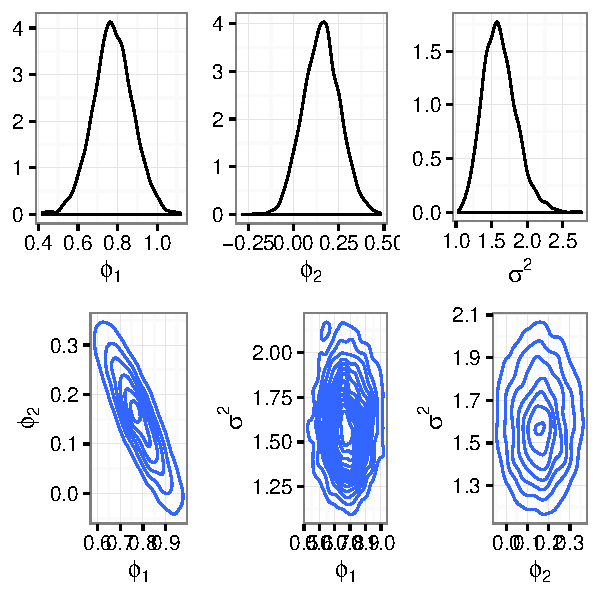
\includegraphics[width=\maxwidth]{figure/AR2MCMC-1} 

\end{knitrout}
\caption{Marginal and bivariate density plots of the MCMC draws. 100,000 draws per parameter were sampled from (\ref{AR2}) via Gibbs MCMC then reduced to 4000 each. Note the strong dependence between the two $\phi$ parameters.}
\end{figure}

The derivation of the MFVB approximation is also in the appendix and each marginal has the same form as the corresponding true conditional distribution above,
\begin{align}
q(\phi_1 | \lambda) &\propto \mathcal{N}(\mu_1^{MF}, \gamma_1^{MF}) \nonumber \\
q(\phi_2 | \lambda) &\propto \mathcal{N}(\mu_2^{MF}, \gamma_2^{MF}) \nonumber \\
q(\sigma^2 | \lambda) &\propto \mathcal{IG}(shape = \alpha^{MF},  scale = \beta^{MF}), \nonumber
\end{align}

where the parameterising vector $\lambda = (\mu_1^{MF}, \gamma_1^{MF}, \mu_2^{MF}, \gamma_2^{MF}, \alpha^{MF}, \beta^{MF})'$.

The MVFB derivation yields the following updating equations for $\lambda$,

\begin{align}
\mu_1^{MF} &= \frac{\alpha^{MF}/\beta^{MF} (\sum_{t=3}^{T} y_t y_{t-1} - \mu_2 \sum_{t=3}^{T} y_{t-1} y_{t-2}) + \tau_1^{-1} \bar{\phi_1}}{\alpha^{MF}/\beta^{MF} \sum_{t=3}^{T} y_{t-1}^2  +  \tau_1^{-1}} \nonumber \\
\gamma_1^{MF} &= \left(\alpha^{MF}/\beta^{MF} \sum_{t=3}^{T} y_{t-1}^2  +  \tau_1^{-1} \right)^{-1} \nonumber \\
\mu_2^{MF} &= \frac{\alpha^{MF}/\beta^{MF} (\sum_{t=3}^{T} y_t y_{t-2} - \mu_1 \sum_{t=3}^{T} y_{t-1} y_{t-2}) + \tau_2^{-1} \bar{\phi_2}}{\alpha^{MF}/\beta^{MF} \sum_{t=3}^{T} y_{t-2}^2  +  \tau_2^{-1}} \nonumber \\
\gamma_1^{MF} &= \left(\alpha^{MF}/\beta^{MF} \sum_{t=3}^{T} y_{t-2}^2  +  \tau_2^{-1} \right)^{-1} \nonumber \\
\alpha^{MF} &=  a + T/2 - 1  \nonumber \\
\beta^{MF} &= b + 1/2 \sum_{t=3}^{T} \left((y_t^2 - ((\mu_1^{MF})^2 + \gamma^{MF}_1) y_{t-1}^2 - ((\mu_2^{MF})^2 + \gamma_2^{MF}) y_{t-2}^2\right) \nonumber \\
&+ 2 \sum_{t=3}^{T} \left(\mu^{MF}_1 \mu^{MF}_2 y_{t-1}y_{t-2} - \mu^{MF}_1 y_{t} y_{t-1} - \mu^{MF}_2 y_t y_{t-2}\right) \nonumber.
\end{align}

The forms of each component are similar to the conditionals derived for Gibbs sampling, with changes coming from linearising the expressions before taking expectations. Notice that all components of $\lambda$ except $\alpha^{MF}$ depend on each other through the expectations in (\ref{mf3}).

The SGA algorithm requires the specification of the approximating family so we make the following assumptions:
\begin{itemize}
\item The optimal marginal distribution for the dependent SGA approximation is the same as the independent MFVB approximation.
\item There is no dependence between either $\phi$ parameter and $\sigma^2$.
\item There is eliptical dependence between $\phi_1$ and $\phi_2$.
\end{itemize}

To determine the form of dependence between $\phi_1$ and $\phi_2$ we fit elliptical copulas to the MCMC draws and determined that the gaussian copula is the best fit by BIC. Gaussian marginals for each $\phi$ and a gaussian copula leads to $\phi_1$ and $\phi_2$ having a bivariate gaussian distribution.

Hence we have the following form for the SGA approximations,

\begin{align}
q(\phi_1, \phi_2) &\sim \mathcal{N}(\mu, \Sigma) \nonumber \\
q(\sigma^2) &\sim \mathcal{IG}(\alpha, \beta). \nonumber
\end{align}

As each parameter in $\Sigma$ can move independently in the SGA algorithm, we instead use the lower triangluar decomposition $L L^T = \Sigma$. This results in the vector $\lambda = (\mu_1, \mu_2, L_{11}, L_{21}, L_{22}, \alpha, \beta)'$, where

\begin{itemize}
\item $\mu_1$: The mean of $\phi_1$,
\item $\mu_2$: The mean of $\phi_2$,
\item $L_{11}, L_{21}, L_{22}$, the three components of $L$, the lower triangular decomposition of $\Sigma$,
\item $\alpha, \beta$, the shape and rate parameters of an Inverse Gamma distribution for $\sigma^2$.
\end{itemize}

The diagonal of $L$ is not forced to be positive so the decomposition is not invariant to sign changes.

We compare three forms of the SGA algorithm, the original algorithm described by \ref{alg:algorithm2}, the reparameterised version described by \ref{alg:algorithm3} and the control variate version described by \ref{alg:algorithm4}. Each version is implemented with $\rho^(m)$ using AdaGrad as in (\ref{adagrad}. 

The reparameterised SGA algorithm requires an auxillay distribution $q(\epsilon)$ and transformation. We use $(\epsilon_1, \epsilon_2)' \sim \mathcal{N}(0, I)$ and $\epsilon_3 \sim \mathcal{U}(0, 1)$. Then make the transformation

\begin{align}
\phi_1 &= \mu_1 + L_11 \epsilon_1 \nonumber \\
\phi_2 &= \mu_2 + L_21 \epsilon_1 + L_22 \epsilon_2 \nonumber \\
\sigma^2 &= Q^{-1}(\epsilon_3, \alpha, \beta) \nonumber
\end{align}

where $Q^{-1}(\epsilon_3, \alpha, \beta)$ is the Inverse Gamma distribution inverse cdf function with shape $\alpha$ and scale $\beta$.

We summarise each algorithm below in table \ref{table} by its estimated parameters, converged value of the ELBO and runtime. Mean Field algorithm runs extremely quickly but can not estimate the dependence between paramters so the converged ELBO is lower than the alternatives, except for the original SGA algorithm. This estimator is extremely noisy and required a value of $S$ of $200$, which slowed computation but it still converged to a lower optima than the variance reduced algorithms. The reparameterised algorithm, SGA-RP, could be run with $S = 5$ leading to its extremely fast runtime. The control variate algorithm, SGA-CV, was run with $S = 50$, and used $20$ draws per iteration to estimate $\hat{a}$.

\begin{table}
\centering
\label{AR2results}
\begin{knitrout}
\definecolor{shadecolor}{rgb}{0.969, 0.969, 0.969}\color{fgcolor}
\begin{tabular}{l|l|l|l|l|l|l|l|l|l}
\hline
  & mu1 & mu2 & L11 & L21 & L22 & alpha & beta & ELBO & Runtime (seconds)\\
\hline
Mean Field & 0.83 & 0.1 & 0.04 & 0 & 0.05 & 50 & 79.7 & -77.7 & 1.3 x 10\textasciicircum{}\{-6\}\\
\hline
SGA & 0.63 & 0.27 & 0.09 & -0.12 & 0.05 & 45.6 & 81.4 & -78.3 & 51.1\\
\hline
SGA-RP & 0.78 & 0.15 & 0.1 & -0.09 & 0.05 & 49.3 & 78 & -76.7 & 4\\
\hline
SGA-CV & 0.77 & 0.15 & 0.09 & -0.09 & 0.05 & 48.5 & 77.6 & -76.9 & 1.3\\
\hline
\end{tabular}


\end{knitrout}
\caption{Parameter estimates, maximised ELBO and runtime of all Variational Bayes algorithms.}
\end{table}

\section{Approximate Forecast Updating}
\subsection{Motivation}
-Slow convergence of MCMC
-Bad scaling to large dimensional models and datasets
-Time/Computational Constraints
-Motivation from short forecast windows
\subsection{Model Selection}
-Overnight/Intermittent MCMC
-Infer model structure from draws
-Have easy parametric form of posterior to work with

\bibliographystyle{asa}
\bibliography{references}



\section{Appendix}
\subsection{AR2 Model}
\end{document}
